\section{\tool}
\label{sec:tool}

\subsection{Goals}
\label{sec:tool:goals}

We identify the broad design goals for a technique to automatically repair
malformed strings or incorrect handling of strings as follows:

% i) identifies the statements which might be vulnerable to string-related errors,
% and are less critical to the functionality of the application such that
% suboptimal behavior might be acceptable,
% iii) generates patches by identifying constraints on the string data and if
% required, tweaks \code{String} API  parameters to regenerate legally correct
% string data,
% iv) optimizes the number of statements to be patched by retaining only the ones
% that need to be protected,  

\myparagraph{(i) High patch fidelity} We require that the patched program must
preserve the intended program behavior, \ie\ the patch must be precise and
should not induce any undesirable control flows in the repaired program.

\myparagraph{(ii) Non-invasive instrumentation} We require that the technique
must ensure no side-effects during normal program execution and activate patches
only when the program is guaranteed to crash.

\myparagraph{(iii) Low system overhead} We desire that the patched program must
incur no runtime overhead during normal program execution and only negligible
overhead in case of failures.

\subsection{Design}
\label{sec:tool:design}

\begin{figure}[t]
\centering
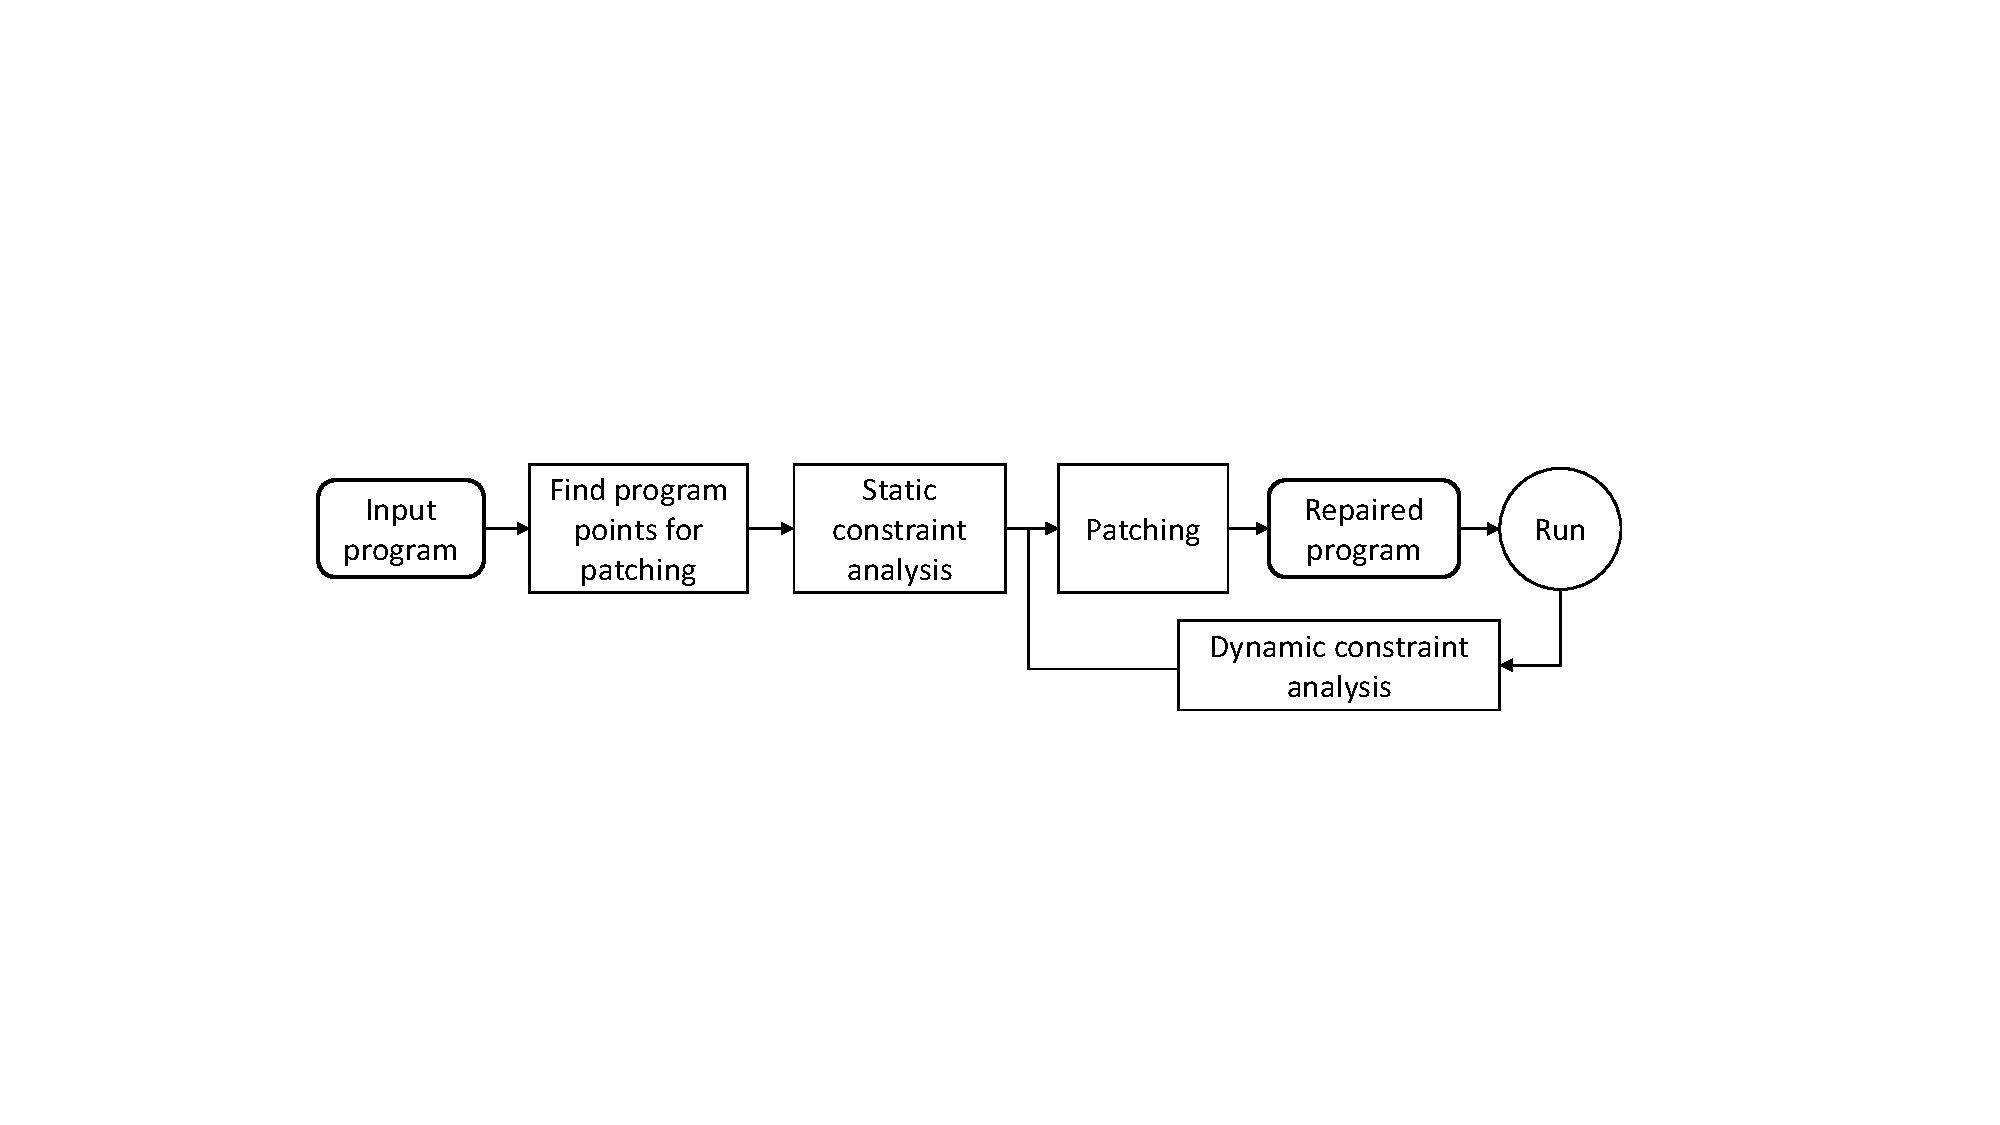
\includegraphics[scale=.38]{images/NewDesignDiagram.pdf}
\caption{\tool\ workflow.}
\label{fig:overallDesign}
\end{figure}

\myparagraph{\underline{Key Idea}} \tool\ leverages precise taint analysis and
call graph analysis to identify program instrumentation points, and builds upon
custom algorithms to generate targeted, high quality patches for repairing
programs with potential runtime exceptions, while still satisfying goals
mentioned in \xref{sec:tool:goals}.

Figure~\ref{fig:overallDesign} shows \tool's workflow, which involves three
main stages. First, \tool\ uses precise program analysis techniques to identify
points of interest, \ie\ string objects or API arguments that must be repaired
to prevent runtime exceptions. In the second stage, \tool\ leverages novel
custom algorithms to generate relevant patches. Specifically, \tool\ performs
intra-procedural static and dynamic analyses to identify and evaluate
constraints on the string objects under consideration. Third, \tool\ uses the
constraints evaluated in the earlier stage to programatically generate and embed
patches inside \texttt{catch} blocks to ensure that they do not get activated
during normal program execution.

\subsubsection{Precise Identification of Instrumentation Points}
\label{sec:tool:stage1}

In this stage, \tool\ leverages a combination of program analyses to accurately
determine the minimum set of points of interest where instrumentation is
required to repair. We list several techniques below that help \tool\ achieve
precision.

\myparagraph{(i) Taint analysis}: The main purpose of taint analysis is to
broadly identify which program statements can be patched (possibly even
suboptimally) without affecting the program control flow, \ie\ affect only
objects that are generated and stay within the application throughout their
lifetime. While this principle is not a binding constraint, it ensures that
\tool's repairing mechanism does not adversely affect critical program behavior.
We specify a generic set of sensitive sources and sensitive sinks for each input
program, to identify critical program paths where a repaired \code{String}
objects (and thus possibly suboptimal) must not flow. For example, \tool\ does
not repair program statements that lie along a control flow path that leads to
an I/O sink, like file system, console, network, GUI, etc.

\begin{table}[t]
\centering
\scriptsize
% \setlength{\tabcolsep}{3pt}
\begin{tabular}{l|l}
\multicolumn{1}{c|}{\textbf{Class}} & \multicolumn{1}{c}{\textbf{Source}}\\
\hline
\code{java.io.InputStream} & \code{read()}\\
\code{java.io.BufferedReader} & \code{readLine()}\\
\code{java.net.URL} & \code{openConnection()}\\
\code{java.util.Scanner} & \code{next()}\\
% \code{javax.servlet.http.HttpServletRequest} & \code{getParameter()}\\
\code{javax.servlet.ServletRequest} & \code{getParameter()}\\
\code{org.apache.http.HttpResponse} & \code{getEntity()}\\
\code{org.apache.http.util.EntityUtils} & \code{toString()}\\
\code{org.apache.http.util.EntityUtils} & \code{toByteArray()}\\
\code{org.apache.http.util.EntityUtils} & \code{getContentCharSet()}\\
\end{tabular}
\caption{Common sensitive sources in \java.}
\label{table:TaintSources}
\end{table}

\begin{table}[t]
\centering
\scriptsize
% \setlength{\tabcolsep}{3pt}
\begin{tabular}{l|l}
\multicolumn{1}{c|}{\textbf{Class}} & \multicolumn{1}{c}{\textbf{Sink}}\\
\hline
\code{java.io.FileOutputStream} & \code{write()}\\
\code{java.io.OutputStream} & \code{write()}\\
\code{java.io.PrintStream} & \code{printf()}\\
\code{java.net.Socket} & \code{connect()}\\
\code{java.io.Writer} & \code{write()}\\
\end{tabular}
\caption{Common sensitive sinks in \java.}
\label{table:TaintSinks}
\end{table}

The taint analysis module take as input the compiled byte code intended to be
repaired, and generates a control flow graph (CFG) identifying program
statements that lie along paths from sensitive sources to sensitive sinks.
Since, \tool\ targets strings in particular, it must support taint propagation
for all \java\ APIs that support string manipulation, including
\code{StringBuffer} and \code{StringBuilder}. All \code{String} objects (whether
generated or assigned) that lie along the tainted path from a sensitive source
to a sensitive sink are marked as \textit{unsafe} to patch. Subsequently, \tool\
does not repair such \code{String} objects. Figures~\ref{table:TaintSources} and
\ref{table:TaintSinks} list some common sensitive sources and sinks for several
classes in \java.

\myparagraph{(ii) Call graph analysis}:

\myparagraph{(iii) Optimizations}:


\ignore{
\paragraph{Identifying Program Statements.} We perform static taint analysis
to identify sensitive data which are leaving the system via database, network
stream, file stream or console. Providing patches to the
statements that manipulate this data would be undesirable, since
activation of the patches in case failures may allow altered sensitive data to
eventually
reach users. Hence, we only mark those program statements which do
not manipulate these data.

\paragraph{Noninvasive Patching.} In case a runtime exception that is thrown
by a statement as a result of a failure is already caught and handled in a
program,
we skip that statement from patching to avoid interfering with the results. Such
statements are identified by analyzing call-graphs and ensuring that no caller
method
in the call-chain handles the exception or its superclass. By embedding the
patches inside
\texttt{catch} blocks, we ensure that they do not get activated during normal
program execution.

\paragraph{Patch Generation.} We first perform an
intra-procedural static analysis
to identify constraints on the string objects under consideration. By
identifying
the type of exceptions that can be thrown in case of a failure, we
develop patches that
regenerate string objects by tweaking \java\ \code{String} API used in
the statements to regenerate legal string objects and by trying to solve the
constraints. In the latter case,
we evaluate the constraints statically if complete information is available at
the compilation-time. Otherwise, the analysis automatically generates
code that performs dynamic analysis to solve the constraints, and then
inserts this code in the generated patches.

\paragraph{Optimizing Instrumentation.} We perform reaching definitions
analysis to skip marked statements
if the string variables that are contained in the statements are already
patched, and the variables
are not redefined along any path that originates from the patched statement.
This analysis reduces
instrumentation points in a program.

\paragraph{Patch Precision.} The precision of a program patch is improved,
firstly, by targeting only strings
for patching which allows us to develop more specialized patches, secondly, by
patching programs very
close to the points of potential failures which avoids unnecessary patching of
other
unaffected variables and their potential
side effects, thirdly, by analyzing the types of exceptions that can be thrown
which
provides valuable insights into
origins of failures, and finally, by considering all the constraints
on the strings. This would result
in a program behavior closed to the intended one in case of a failure.

\paragraph{Reduced Overhead.} The side-effect of non-invasive patches is that
they do not interfere during
normal execution which results in no runtime overhead. Even when they get
activated in case of failures,
they still cause negligible overhead since we perform no analysis during runtime
except if required resolve the dynamic constraints.
As our study reveals~\xref{sec:evaluation} the constraints are typically few and
simple, making
the dynamic analysis light-weight.
}

